\documentclass[%
oneside,                 % oneside: electronic viewing, twoside: printing
final,                   % draft: marks overfull hboxes, figures with paths
10pt]{article}

\listfiles               %  print all files needed to compile this document

%\usepackage[a4paper, total={6in, 8in}]{geometry}
\usepackage[totoc]{idxlayout}   % for index in the toc
\usepackage[nottoc]{tocbibind}  % for references/bibliography in the toc

\usepackage{relsize,makeidx,color,setspace,amsmath,amsfonts,amssymb}
\usepackage[table]{xcolor}
\usepackage{bm,ltablex,microtype}
\usepackage{comment} 
\usepackage[pdftex]{graphicx}

\usepackage{fancyvrb} % packages needed for verbatim environments

\usepackage[T1]{fontenc}
%\usepackage[latin1]{inputenc}
\usepackage{ucs}
\usepackage[utf8x]{inputenc}

\usepackage{lmodern}         % Latin Modern fonts derived from Computer Modern


\usepackage{pgfplotstable, booktabs}

\pgfplotstableset{
    every head row/.style={before row=\toprule,after row=\midrule},
    every last row/.style={after row=\bottomrule}
}





% Hyperlinks in PDF:
\definecolor{linkcolor}{rgb}{0,0,0.4}
\usepackage{hyperref}
\hypersetup{
    breaklinks=true,
    colorlinks=true,
    linkcolor=linkcolor,
    urlcolor=linkcolor,
    citecolor=black,
    filecolor=black,
    %filecolor=blue,
    pdfmenubar=true,
    pdftoolbar=true,
    bookmarksdepth=3   % Uncomment (and tweak) for PDF bookmarks with more levels than the TOC
    }
%\hyperbaseurl{}   % hyperlinks are relative to this root

\setcounter{tocdepth}{2}  % levels in table of contents

% --- fancyhdr package for fancy headers ---
\usepackage{fancyhdr}
\fancyhf{} % sets both header and footer to nothing
\renewcommand{\headrulewidth}{0pt}
\fancyfoot[LE,RO]{\thepage}
% Ensure copyright on titlepage (article style) and chapter pages (book style)
\fancypagestyle{plain}{
  \fancyhf{}
  \fancyfoot[C]{{\footnotesize \copyright\ 1999-2018, "Computational Physics I FYS3150/FYS4150":"http://www.uio.no/studier/emner/matnat/fys/FYS3150/index-eng.html". Released under CC Attribution-NonCommercial 4.0 license}}
%  \renewcommand{\footrulewidth}{0mm}
  \renewcommand{\headrulewidth}{0mm}
}
% Ensure copyright on titlepages with \thispagestyle{empty}
\fancypagestyle{empty}{
  \fancyhf{}
  \fancyfoot[C]{{ }}
  \renewcommand{\footrulewidth}{0mm}
  \renewcommand{\headrulewidth}{0mm}
}

\pagestyle{fancy}


% prevent orhpans and widows
\clubpenalty = 10000
\widowpenalty = 10000

% --- end of standard preamble for documents ---


% insert custom LaTeX commands...

\raggedbottom
\makeindex
\usepackage[totoc]{idxlayout}   % for index in the toc
\usepackage[nottoc]{tocbibind}  % for references/bibliography in the toc
\usepackage{listings}
\usepackage[normalem]{ulem} 	%for tables
\useunder{\uline}{\ul}{}
\usepackage{hyperref}
\usepackage[section]{placeins} %force figs in section

\usepackage{natbib}

\usepackage[toc,page]{appendix} % appenix


%-------------------- end preamble ----------------------

\begin{document}

% matching end for #ifdef PREAMBLE

\newcommand{\exercisesection}[1]{\subsection*{#1}}


% ------------------- main content ----------------------



% ----------------- title -------------------------

\thispagestyle{empty}

\begin{center}
{\LARGE\bf
\begin{spacing}{1.25}
Classification and Regression, from linear and logistic regression to neural networks
\end{spacing}
}
\end{center}

% ----------------- author(s) -------------------------

\begin{center}
{\bf Johan Nereng}
\end{center}

    \begin{center}
% List of all institutions:
\centerline{{\small Department of Physics, University of Oslo, Norway}}
\end{center}
    
% ----------------- end author(s) -------------------------

% --- begin date ---
\begin{center}
Nov 13, 2019
\end{center}
% --- end date ---

\vspace{5cm}
\begin{abstract}
-------
\end{abstract}
\newpage




\textit{\textbf{----}} \newline


\textit{\textbf{Authors' comment:} ---- painfully obvious that I cannot correctly code all the methods in a vacuum - especially in the case of neural networks, were there are fewer "right" answers, and more trial and error, need to spend more time at CCSE, so that I may discuss code and results with co-students. Need to have more condensed and in many cases less detailed descriptions of my simulations and results. }
\newpage

\section{Introduction}
\subsection{Qualitative response modeling}
This project's main focus is modeling qualitative response variables. Where quantitative response variables models for continuous outputs, classifiers model such as logistic regression models for probabilities that a data entry belongs in a certain category. Due to this, the regression methods used for numerical output values are ill suited. If one insist on using for example least squares in categorical prediction, one runs into the problem of ordering of responses and category gaps (explained in detail in  \citep{2017introstatlearn}[p.130]). Neural networks on the other hand are flexible in this regard. The basic structure of the network, explained in more detail in the methods sections, remains the same for any type of regression. What changes however are the activation functions
\hyperref[Section_Methods]{methods sections}
\hyperref[Section_Results]{Results}
\hyperref[Section_Discussion_of_results]{discussion of results}
\hyperref[Section_Conclusions]{conclusions}

\hyperref[Section_M_Scaling]{Scaling}
\hyperref[Section_M_Logreg]{Logistic Regression}
\hyperref[Section_M_NN]{Neural Networks}
\hyperref[Section_M_Codeimpl]{Code Implementation}
\hyperref[Section_M_eval]{Evaluating The Implementation}

\textit{autoths: left right mult. confusing in looking at notes, example code and nielsens book}
Regression vs classification
crossvalidation
mean-squared error and/or the R2
or the accuracy score (classification problems) 

Assumes prior knowledge of fundamentals of machine learning, such as what a design matrix, predictors and response is.

A network such as this is a universal approximator, which means that it can approximate any suitably smooth with arbitrary accuracy \citep{MLMurphy}[p.564].
\section{Methods} \label{Section_Theory}

\subsection{Logistic Regression for two classes} \label{Section_M_Logreg}
Logistic regression models the probability that a qualitative response falls within a category. In the case of two mutually exclusive categories or classes, such as "True" ($Y=1$) and "False" ($Y=0$), this translates to modeling the relationship between the probability of $Y=1$ given $X$ as $P(Y=1|X;\beta)=p(X;\beta)$, using the \textit{logistic function} \eqref{eq:logfunc} \citep{2017introstatlearn}[p.132], which due to mutual exclusivity, models $Y=0$ as a function of $X$, or $P(Y=0|X)=p(X';\beta)$, as $1-p(X;\beta)$.
\begin{equation}
p(Y=1|X, \bm{\beta})= p(\bm{X};{\beta})=\frac{e^{\bm{\beta}\bm{X}}}{1+e^{\bm{\beta}\bm{X}}}
\label{eq:logfunc}
\end{equation}
where $\bm{\beta}=[\beta_0, \beta_1, ... \beta_p]$, $\bm{X}=[1,X_1, X_2, ... X_p]$, and $p$ is the number of predictors that the the binary response $Y$ is modeled upon. When fitting the model (estimating the $\beta$ coefficients) to a data set $\mathcal{D}=\{y_i,\bm{x}_i\}_{i=1}^n$, of $n$ observations, the desired fit is the one where the predicted probabilities of $p(\bm{x}_i)$  most precisely corresponds to $y_i$. In other words, one seeks the model which has the highest probability of predicting the data set, which is achieved by utilizing the \textit{maximum likelihood} method \eqref{eq:max_likelihood}\citep{2017introstatlearn}[p.133]. 



\begin{equation}
P(\bm{\beta})=\displaystyle\prod_{i:y_i=1}p(\bm{x}_i; \bm{\beta}) \displaystyle\prod_{i':y_{i'}=0}(1-p(\bm{x}_{i'}; \bm{\beta}))
\label{eq:max_likelihood}
\end{equation}

Taking the log of the maximum likelihood, one obtains the log-likelihood. The (reordered) negative log-likelihood constitutes the cost function, $\mathcal{C}(\hat {{\beta}})$ \eqref{eq:cost_log} \citep{HastieTrevor2009TEoS}[p.120] (in Hastie et al, the log-likelihood is maximized) of the logistic regression, or the \textit{cross entropy}. When minimized, this convex function yields the desired $\beta$ estimates.

\begin{equation}
\mathcal{C}(\bm{\beta})=-\sum_{i=1}^n \left(y_i({\bm{\beta}}\bm{x}_i)-log(1+e^{{\bm{\beta}}\bm{x}_i})\right)
\label{eq:cost_log}
\end{equation}

\subsection{Gradient Decent}  \label{Section_M_GD}
The minimization of a cost function may in some cases be carried out analytically, for example when using least squares error. For some cost function however, the analytic expression may be inconvenient to use. Factors such as the size of a matrix which requires inverting may be to computationally intensive, and in yet other cases, close form solutions are entirely unavailable. For problems such as these, numerical methods for obtaining the desired model fit is instead applied. One such method is the gradient descent (GD) \eqref{eq:GD} \citep{MLMurphy}[p.247], also known as steepest descent. When utilizing GD, one makes an initial guess for $\bm{\beta}$, evaluates the gradient, $\bm g$ of the cost function in order to obtain an estimate closer to the desired minimizing value. This process is then iteratively repeated till the sufficient convergence of the coefficients is reached. In order to not overshoot the $k+1$'th estimate, a \textit{learning rate} of $\eta$ is applied to the gradient - which may also serve to lengthen the step in an iteration. The value of the learning rate can either be fixed, usually by trial and error, such that it works well for the problem at hand, or it may be adapted to each step. 

\begin{equation}
\bm{\beta}_{k+1}=\bm{\beta}_{k}-\eta_k  \bm g (\bm{\beta}_k)
\label{eq:GD}
\end{equation}

A regularization parameter, $\lambda $, is often added to the gradient in an extra term, effectively modifying the gradient descent (and SGD), which effectively reduces the growth of the weights, thus reducing overfitting to the training data.
\begin{equation}
\bm{\beta}_{k+1}=\bm{\beta}_{k}-\eta_k  \bm g (\bm{\beta}_k)(1+\lambda)
\end{equation}

For logistic regression, $\bm g$, may be expressed as: \citep{MLMurphy}[p.247]:
\begin{equation}
\bm g (\bm \beta)= \frac{\partial \mathcal{C}(\bm{\beta})}{\partial \bm \beta}= -\hat{X}^T(\bm y-\bm p )
\end{equation}
Where $\hat{X}$, is the design matrix, and $\bm p$ a vector with elements $p(y_i|x_i;\bm \beta)$. \newline

A common improvement on GD is the stochastic gradient descent (SGD), which involves splitting the data into min batches, then randomly selecting one batch at a time from which to compute the gradient. More detailed information is available in literature such as Kevin P. Murphy's book on machine learning \citep{MLMurphy}[p.262].

\subsection{Neural Networks} \label{Section_M_NN}
\textit{For simplicity's sake, matrices are denoted without bold font or hats from here on forwards.} The feed forward neural network (FFNN), or multi-layer perceptron model (MLP), is an artificial neuron network consisting of an ordered series of regression models with connected inputs and outputs \citep{MLMurphy}[p.563]. The network consists of $L$ layers, with  a number of neurons (regression models), or nodes, in each layer. The neurons are not necessarily of the same type, as one can for example use logistic regression models for all nodes but the ones in $L$, which could be linear regression models if the problem is a regression problem. The outputs, $a^1$, of the $M_1$ nodes in layer $l=1$ (one), the input layer, are fed to the nodes in layer $l=2$, and so on, until the outputs, $a^{L-1}$, from layer $l=L-1$ is fed to layer $l=L$, the output layer. Outputs from layer $L$, $a^L$ are the network's outputs, and predict the target(s) of the model. The layers in-between layer $1$ and layer $L$, are deterministic functions of the input, and are called hidden layers.  Each node in each layer uses weights for each input, similar to the coefficients  corresponding to the predictors described in the \hyperref[Section_M_Logreg]{logistic regression subsection}. In addition, each node has it's own \textit{bias}, $b$, which regulates the output tendency of neuron. The sum of the weighted inputs and the bias, $z$, is usually called the activation of the neuron, not to be confused with it's output. The output is however a function of the activation, such that $a^l=f^l(z^l)$, where $f(z)$ is called an activation function. \newline

\textit{The remaining subsections on neural networks are based on the informative and well written book by Michael Nielsen book \citep{Nielsen15} (using a slightly different matrix indexation than what this project does), and lectures notes in   FYS-STK4155 \cite{MHJ_NN}}.
\subsubsection{Feed forward}
The propagation of neuron outputs in the network, resulting in prediction, is called feed forward. The network used in this project is set up such that it takes  $n_{inputs}$ observations, of $n_{predictors}$ predictors, thus working through the entirety of the data in one go. As with other regression methods, the design matrix $X$ ($n_{inputs} \times n_{predictors}$) is the input, which in the end outputs a matrix $ y$ ($n_{inputs} \times n_{targets}$) of predicted values for the $n_{targets}$ targets. By arranging the weights of layer $l$, $w^l$ ($M_{l-1} \times M_l$), the activations of layer $l$ is calculated by $z_l=X w^l$ ($n_{inputs} \times M_l$). Taking $a^l=f^l(z^l)$ ($n_{inputs} \times M_l$), means that $a^l$ holds the output for every neuron in $l$. 

\subsubsection{Cost function and backpropagation} \label{Section_M_NN}
Once $a^L$ is obtained through the feed forward process, the network has made a prediction on the target(s), $y$, for each of the $n_{inputs}$ observations. However, unless one has divine insights, initiating the weights and biases such that $a^L \approx y$ with sufficient accuracy is unlikely. The quality of these  predictions is quantified by the cost function $C(w,b)$, which as indicated is a function of the weights and biases of network. The effect on prediction quality when adjusting $w$ and $b$ is thus measurable by the cost function, which, as in the case of the logistic regression, is to be minimized. In the case of FFNNs, this is done through backpropagation, which is the process of calculating the error of each layer, \eqref{eq:BP1} and \eqref{eq:BP2}, and the gradient of the cost, $\nabla C$, function w.r.t the biases \eqref{eq:BP3} and weights \eqref{eq:BP4}. 
\begin{align}
\label{eq:BP1} &\delta_L=\nabla_a C \odot  f' (z^L) \\  
\label{eq:BP2} &\delta_l=\delta^{l+1}(w^{l+1})^T \odot  f' (z^l)\\ 
 \label{eq:BP3} &\frac{\partial C}{\partial b^l} =\delta^l\\ 
\label{eq:BP4} &\frac{\partial C}{\partial w^l} =(a^{l-1})^T \delta^l 
\end{align}

Having obtained the gradient $\nabla C$, \hyperref[Section_M_GD]{gradient decent} is applied in order to calculate new weights and biases. Once the weights and biases are updated, a new feed forward process is initiated, followed by backpropagation and corresponding adjustments of parameters until the cost function is sufficiently minimized or the number of iterations (feed forward + backpropagation) is reached. 

\subsubsection{Neural network for classification}  \label{Section_M_NNclass}
In the logistic regression case, this project did not use one hot encoding - using  cross entropy ensures equal importance of both target options when training. For the NN implementation however, one-hot encoding is used, along with cross entropy \eqref{eq:cost_log} as the cost function. As the one-hot encoding means that the network is expected to output two values, representing the likelihood of each of the two categories for each data point, the activation function of the output layer is the softmax function \eqref{eq:softmax} (output of neuron $j=1,2$ in $L$), which normalizes the sum of the outputs to one.  

\begin{equation}
a_j^L= \frac{e^{z_j^L}}{\sum e^{z^L}}
\label{eq:softmax}
\end{equation}
Using the cross entropy as the cost function, sigmoid for hidden layer(s), and softmax as the activation for layer $L$, means that the backpropagation equations \eqref{eq:BP1}-\eqref{eq:BP4} for the two last layers of network are:
\begin{align*}
&\delta_L=a_L-y \\   
&\delta_{L-1}=\delta_L(w^{L})^T \odot  a_{L-1} \odot (1- a_{L-1})\\ 
&\frac{\partial C}{\partial b^L} =\delta^L\\ 
&\frac{\partial C}{\partial w^L} =(a^{L-1})^T \delta^{L}  \\
&\frac{\partial C}{\partial b^{L-1}} =\delta^{L-1}\\ 
&\frac{\partial C}{\partial w^{L-1}} =(a^{L-2})^T \delta^{L-1} 
\end{align*}
It's worth noting that in the output error, when using softmax with cross-entropy, the $f'(z)$ term cancels with parts of the derivative of $C$ w.r.t $a$.
\subsubsection{Neural network for regression}  \label{Section_M_NNregression}
In this project, the neural network for regression is set up using the quadratic cost, with $tanh (z)$ as activation function in hidden layer(s), and with $f(z^L)=z^L$, the identity activation, as activation for the output layer. Due to the change in activation functions, the backpropagation changes slightly, however, as the cost function is also changed, the output error remains the same.

\begin{align*}
&\delta_{L-1}=\delta_L(w^{L})^T    \odot (1-tanh(z_{l-1}^2)) \\ 
\end{align*}

\subsection{Implementation, pre-processing data, testing, and evaluation}
Logistic regression for classification is implemented in it's own program using python 3.7.5. The program also uses functionalities from scikit-learn \cite{sklearn} for splitting data into test and training sets, metrics such as producing a confusion matrix, and scaling functions. A neural network for classification is also implemented, building on the template provided in the lecture slides on neural networks from the course FYS-STK4155 \cite{MHJ_NN}, using the activation functions and cost function as described in the subsection on \hyperref[Section_M_NNclass]{neural networks for classification}. 

\subsubsection{Pre-processing of data}  \label{Section_M_PP}
As the credit card data (and to some extent the cancer data) is skewed ($22\%$ default), to some extent faulty, and in general not processed for regression, pre-processing of the data is required in order to make reasonable model predictions. First, invalid entries  in the categorical predictors are removed from the data all together - such as entries with a value corresponding to another marital status than married (1), single (2) or other (3)]. Then, the categorical predictors; gender, education, and  marital status are one-hot encoded, as it is undesirable to train the model on the assumption that the options for each category have some "distance" between them, which is equal for say  married (1) and single (2), and single(2) and other (3). As it is desirable to limit the number of predictors, the remaining categorical predictors are assumed to not suffer in the same extent from the equal-distance problem and are not one-hot encoded. Having removed some entries and reshaped the design matrix,  it is then standardized (using scikit-learn's standard scaler) by substracting the mean of each predictor and scaling to unit variance. The data is then split into testing and training data, using a stratified split (scikit-learn), ensuring integrity of target category ratio in training and test sets. Lastly, the training data is up-sampled using Smote from imbalanced-learn \cite{imblearn} in order  prevent the model from over-training on the over represented non-default case.

\subsubsection{Model evaluation and quality measurements}
In order to ascertain the quality of the classifiers in this project, accuracy score \eqref{eq:accuracy}, area (ratio) score \eqref{eq:area}, and (intermittently ), confusion matrixes are used. 

\begin{equation}
\text{Accuracy}=\frac{\sum_{i=1}^{i=n}I(t_i=y_i)}{n}
\label{eq:accuracy}
\end{equation}
Where $I$ is the indicator function.
\begin{equation}
\text{Area ratio score}=\frac{\text{Area between model curve and baseline curve}}{\text{Area between optimal model curve and baseline curve}}
\label{eq:area}
\end{equation}
Where the curves in question are the curves obtained in a gains analysis. 

\subsubsection{Initial testing of the logistic regression implementation}
Initial testing of the logistic regression implementation (using both GD and SGD) is carried out on data from the breast cancer set available through scikit-learn, which contains 569 data points with 30 predictors and targets ($212$ WDBC-Malignant, $ 357$ WDBC-Benign). The program features an option to plot (set plot=True in the function call for GD/SGD) the cost function vs. number of iterations/epochs - which shows that the cost function decreases with iterations/epochs. Before training, the data set is scaled using scikit-learn's standard scaler (without any additional pre-processing), and split into test (1/3) and training (2/3) sets. In addition, scikit-learn's logistic regression model is fitted and used to confirm the integrity of the algorithm developed for this project. Based on comparison of area and accuracy scores as well as confusion matrices (\hyperref[APP_1]{see appendix 1}), the implementation is deemed successful.

\subsubsection{Initial testing of neural network implementation}
A neural network with one hidden layer, with a number of nodes equal to the mean between input and output, is now tested on the same data set as when testing the logistic regression implementation, using both smote and scaling. The SGD in the neural network is set to use 1500 epochs with batch size 20, and $\eta=0.1$, and $\lambda=0.0$. This produced an area ratio score of $0.87$ (where as the logistic regression program scored $0.97$). The plot of the cost function \hyperref[APP_1]{(see appendix 1)}, shows that the network minimizes the cost function. Based on these indications, the implementation is deemed successful.

\subsubsection{Logistic regression on credit card data}
Having confirmed the integrity of the implementation, the project now moves on to a brief evaluation of the importance of \hyperref[Section_M_PP]{pre-processing}, while simultaneously establishing their connection to evaluation measurements (accuracy and area score) in skewed data sets when using logistic regression. In order to do so, the credit card data is loaded with outlier-removal and one-hot encoding, and fitted with the logistic regression program (using GD with iterations=$5000$, $\eta=0.1$) without application of stratified split, smote and scaling. Similar fits, with scaling, with smote and scaling, and with smote, scaling and stratified split, is then carried out.

\subsubsection{Neural network on credit card data}
The neural network implementation is now used to predict on the credit card data. The conclusions reached under \hyperref[Section_Discussion_of_results]{discussion of results} on pre-processing from the logistic regression case it is assumed to be applicable for the neural network - although this has not been tested. The credit card data is loaded using outlier removal, one-hot encoding (also on the target in this case), scaling,  and smote. As was the case under the initial test of the neural network, the number of nodes in the hidden layer corresponds to the average between the number of nodes in the input layer and the number nodes in the output layer - $16$ (the credit card data, after one-hot encoding, has $29$ predictors and $2$ targets). First, a gridsearch over batch size and number of epochs for the SGD is carried out, using $\eta=0.1$ and $\lambda=0.1$, followed by an additional gridsearch using $\eta=0.1$ and $\lambda=1.0$. Then, in order to visualize the relationship between the four paramters (epochs, batch size, $\eta$, $\lambda$), an additional gridsearch over values for the regularization parameter $\lambda$ and learning $\eta$ is made, using $1000$ epochs, with batch size $1000$ . All gridsearches use area ratio score as their primary evaluation measurement, as the logistic regression section showed how misleading accuracy can be in the case of skewed data.

\subsubsection{Neural network on Franke's Frunction}
The neural network is modified in accordance with the back-propagation alterations described in the subsection on  \hyperref[Section_M_NNregression]{neural networks for regression}, such that the network (with one hidden layer) may be used for regression when the target has a numerical value. In order to evaluate it's performance, a $30 \times 30$ xy-grid for $x,y\in [0,1]$ using Franke's function \cite{P1_JN} is generated and used to set up a design matrix corresponding to $p=5$ predictors on the form [$x,y,xy,x^2,y^2,xy, ...$]. The predictors are then scaled to a range of $0,1$, with no further pre-processing as most data pre-processing methods for classification do not apply. The network is first trained and tested on the same $30 \times 30$ grids, before being trained and tested on split data set -  it's MSE compared with the OLS model from scikit-learn. The regression is done using batch size $50$ with $1000$ epochs, and a grid search for $\eta$ and $\lambda$, recording the lowest MSE.

\section{Results} \label{Section_Results}
\subsubsection{Logistic regression on credit card data}\label{results_evaluation_pp}
\paragraph{Figure \ref{fig:logreg_no_pp}} shows the gains chart produced by the logistic regression program on the credit card data with no other pre-processing of the data than one-hot encoding and removal of outliers (accuracy$=0.78$, area ratio$=0.00$ - row one table \ref{table:PP_scores}). As the plot suggests, and the area ratio score shows, the model performs similar to the random classifier.

\paragraph{Figure \ref{fig:logreg_best_pp}}  shows the gains chart associated with the highest area ratio ($0.46$) from table \ref{table:PP_scores}. The figure indicates that the model significantly outperforms the random classifier, while not matching optimal model performance.

\paragraph{Table \ref{table:PP_scores}} shows the accuracy and area ratio score for logistic regression with GD ($5000$ iterations and $\eta=0.1$) for different levels of pre-processing - showing that $0.44$ area ratio outlier removal, one-hot, scaling, and smote produce the highest area ratio score of $0.46$. In addition, the table suggests that scaling may be the most important pre-processing in the case of the credit card data. 
\begin{figure}[!h]
        \centering 
         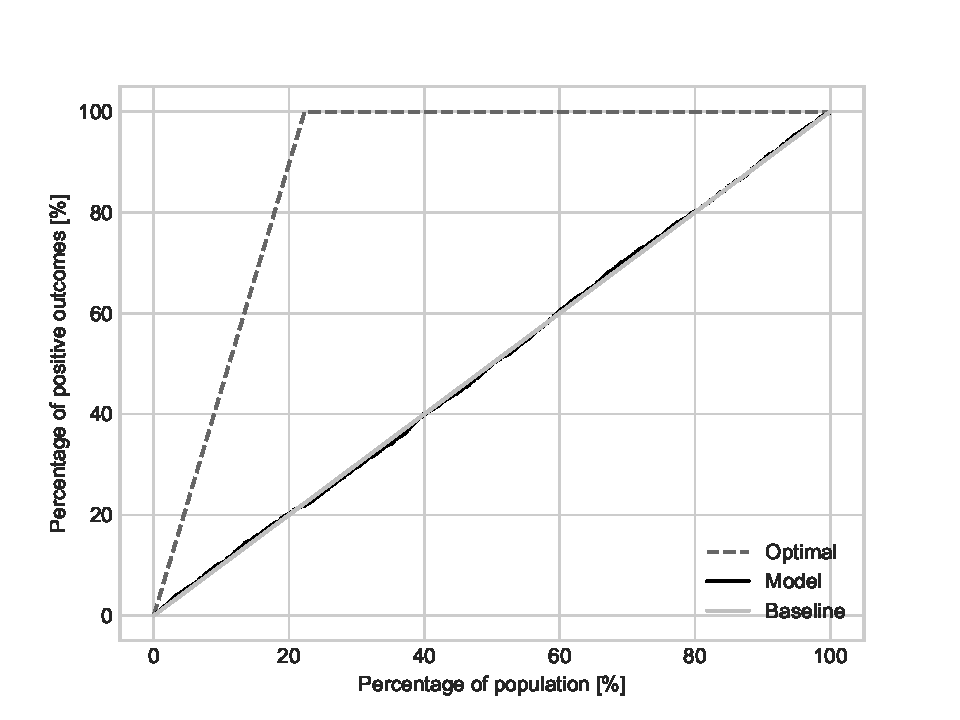
\includegraphics[scale=0.5]{../Results/CC_logreg_no_pp/gains_gd.pdf} 
        \caption{Gains plot for logistic regression using GD with $5000$ iterations and $\eta=0.1$ on credit card data, no pre-processing of data other than one-hot encoding. }
        \label{fig:logreg_no_pp}   
\end{figure}  

\begin{figure}[!h]
        \centering 
         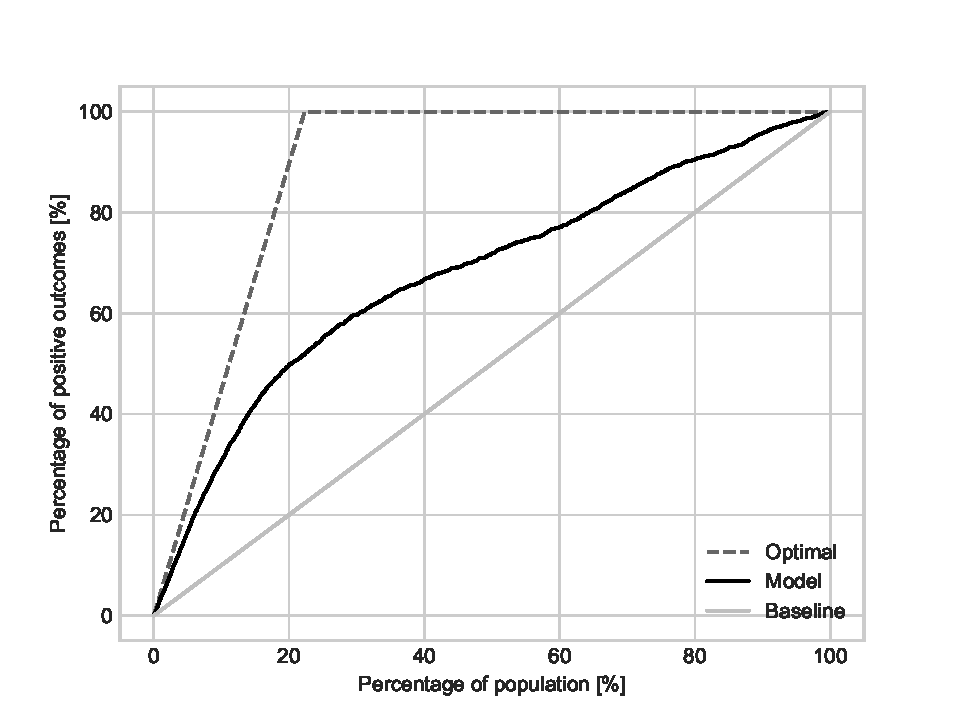
\includegraphics[scale=0.5]{../Results/CC_logreg_scaling_smote/gains_gd.pdf} 
        \caption{Gains plot for logistic regression using GD with $5000$ iterations and $\eta=0.1$ on credit card data, using outlier removal, one-hot, scaling and smote. }
        \label{fig:logreg_best_pp}   
\end{figure}  

\begin{table}[h!]
\begin{center}
\begin{tabular}{lll}
\hline
 Pre-processing  & Accuracy score & Area ratio score      \\
\hline
 Outlier removal, one-hot               & $ 0.78 $ & $0.00$ \\
 Outlier removal, one-hot, scaling               & $  0.60 $ & $0.44$ \\
 Outlier removal, one-hot, scaling, smote  &$0.58$ & $0.46$  \\
 Outlier removal, one-hot, scaling, smote, stratified split    & $0.57$ & $0.44     $   \\
 Outlier removal, one-hot, smote, stratified split    & $0.78$ & $-0.02 $ 
   \\  
\hline
\end{tabular}
\end{center}
\caption{Logistic regression on credit card data; accuracy and area ratio score as functions of different levels of pre-processing (GD with $5000$ iterations and $\eta=0.1$)}
\label{table:PP_scores}
\end{table}
\subsubsection{Neural network on credit card data}

\paragraph{Figure \ref{fig:NN1_grid_epoch}} shows a gridsearch over epochs and batch sizes, for $\eta=0.1$ and $\lambda=0.1$, using outlier removal, one-hot encoding, scaling and smote. The figure indicates that  $500$ epochs and batch sizes of $500$, and  $1000$ epochs and batch sizes of $1000$, yield the best area ratio score ($0.42$).

\paragraph{Figure \ref{fig:NN1_grid_epoch_highl}} shows a gridsearch over epochs and batch sizes, for $\eta=0.1$ and $\lambda=0.1$, using outlier removal, one-hot encoding, scaling and smote. The figure indicates that  $500$ epochs and batch sizes of $1500$, and  $1000$ epochs and batch sizes of $2000$, yield the best area ratio score ($0.43$).

\paragraph{Figure \ref{fig:NN1_grid_eta}}
shows a gridsearch over  $\eta$ and $\lambda$, using $1000$ epochs over a batch size of $1000$ using outlier removal, one-hot encoding, scaling and smote. The figure indicates that  $\eta=0.1$ and $\lambda=0.001$, and $\eta=0.1$ and $\lambda=1.0$, yield the best area ratio score ($0.43$)e.



\begin{figure}[!h]
        \centering 
         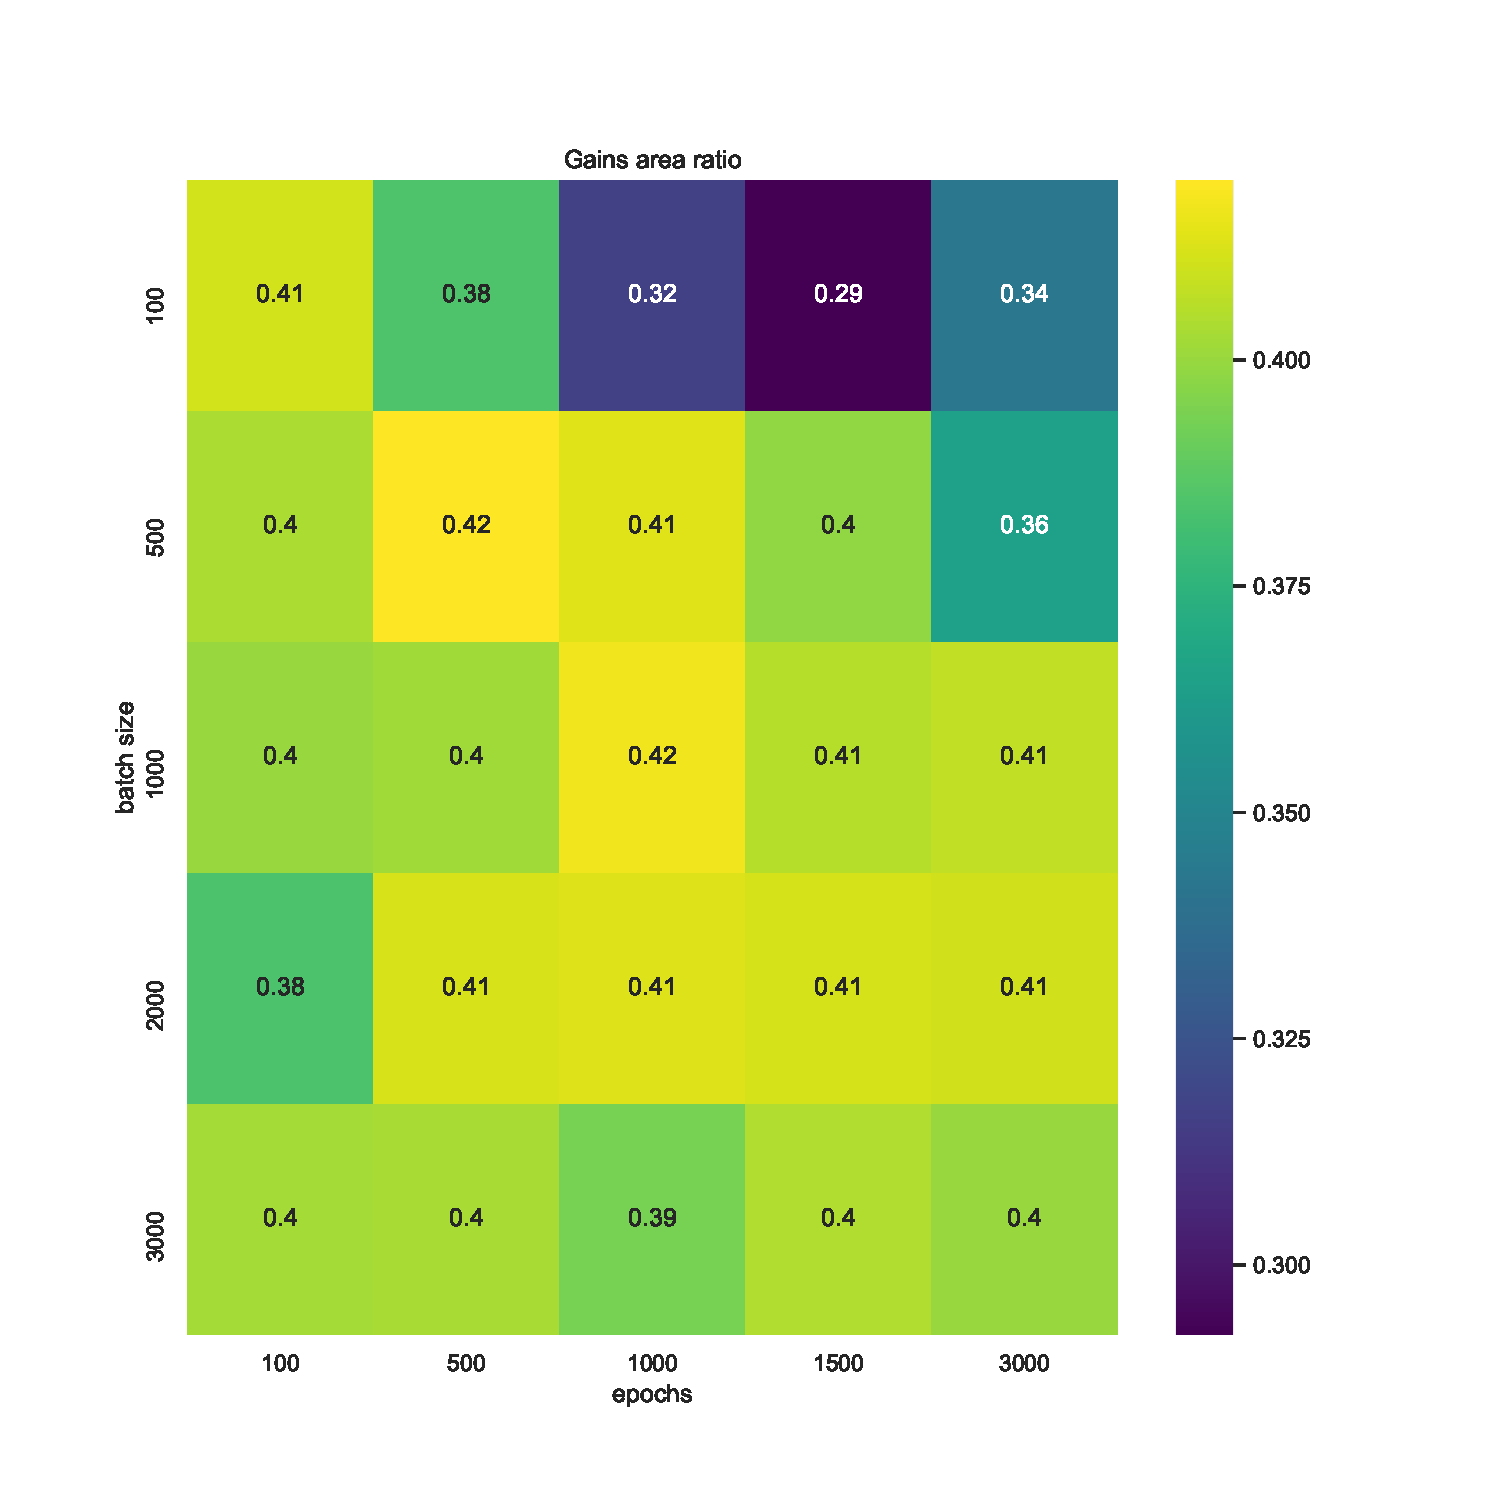
\includegraphics[scale=0.5]{../Results/CC_NN_gridsearch/gridsearch_NN_area_epocs.pdf} 
        \caption{Gridsearch showing area ratio score for a number of epochs and batch sizes using  values of $\eta=0.1$ and $\lambda=0.1$.}
        \label{fig:NN1_grid_epoch}   
\end{figure}  

\begin{figure}[!h]
        \centering 
         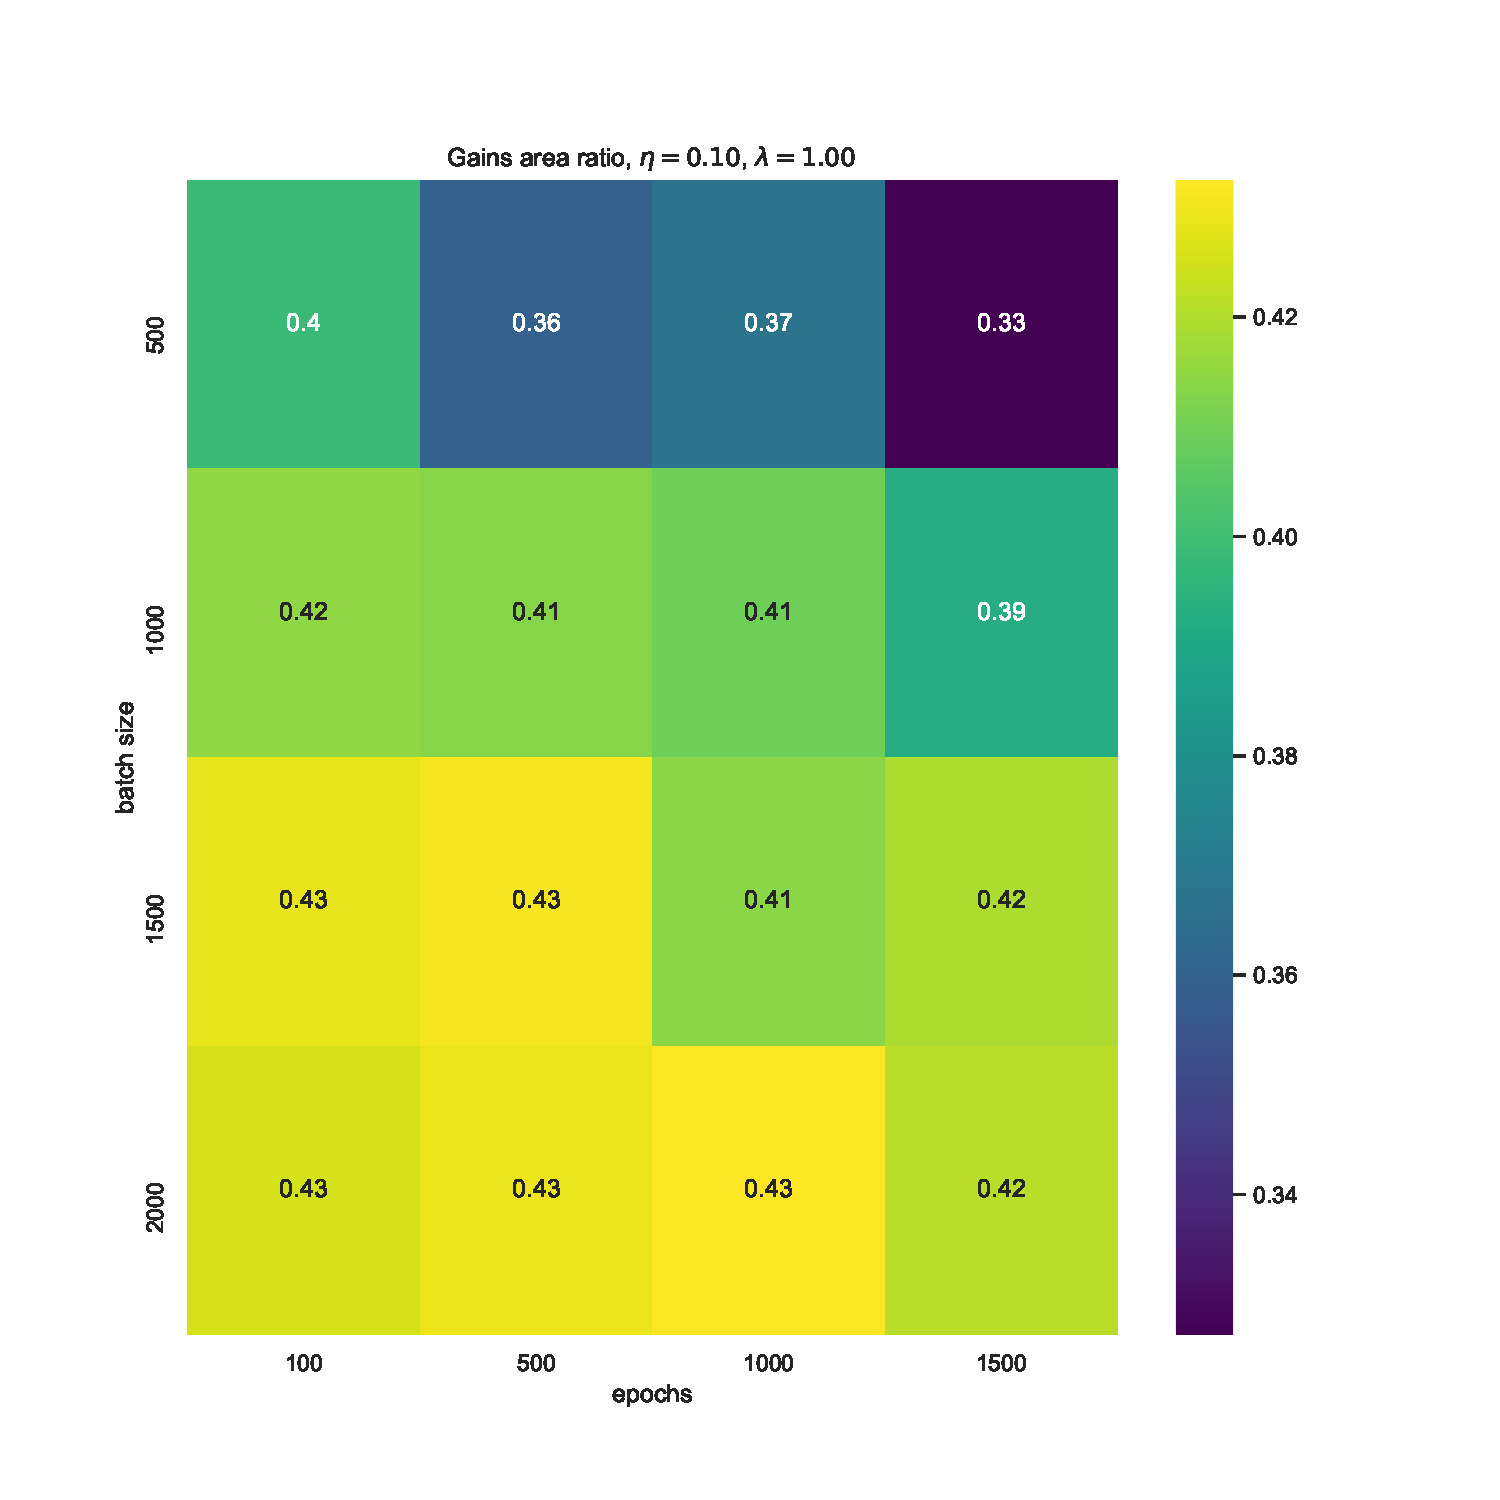
\includegraphics[scale=0.5]{../Results/CC_NN_gridsearch/gridsearch_NN_area_highlambda.pdf} 
        \caption{Gridsearch showing area ratio score for a number of epochs and batch sizes using  values of $\eta=0.1$ and $\lambda=1.0$.}
        \label{fig:NN1_grid_epoch_highl}   
\end{figure}  

\begin{figure}[!h]
        \centering 
         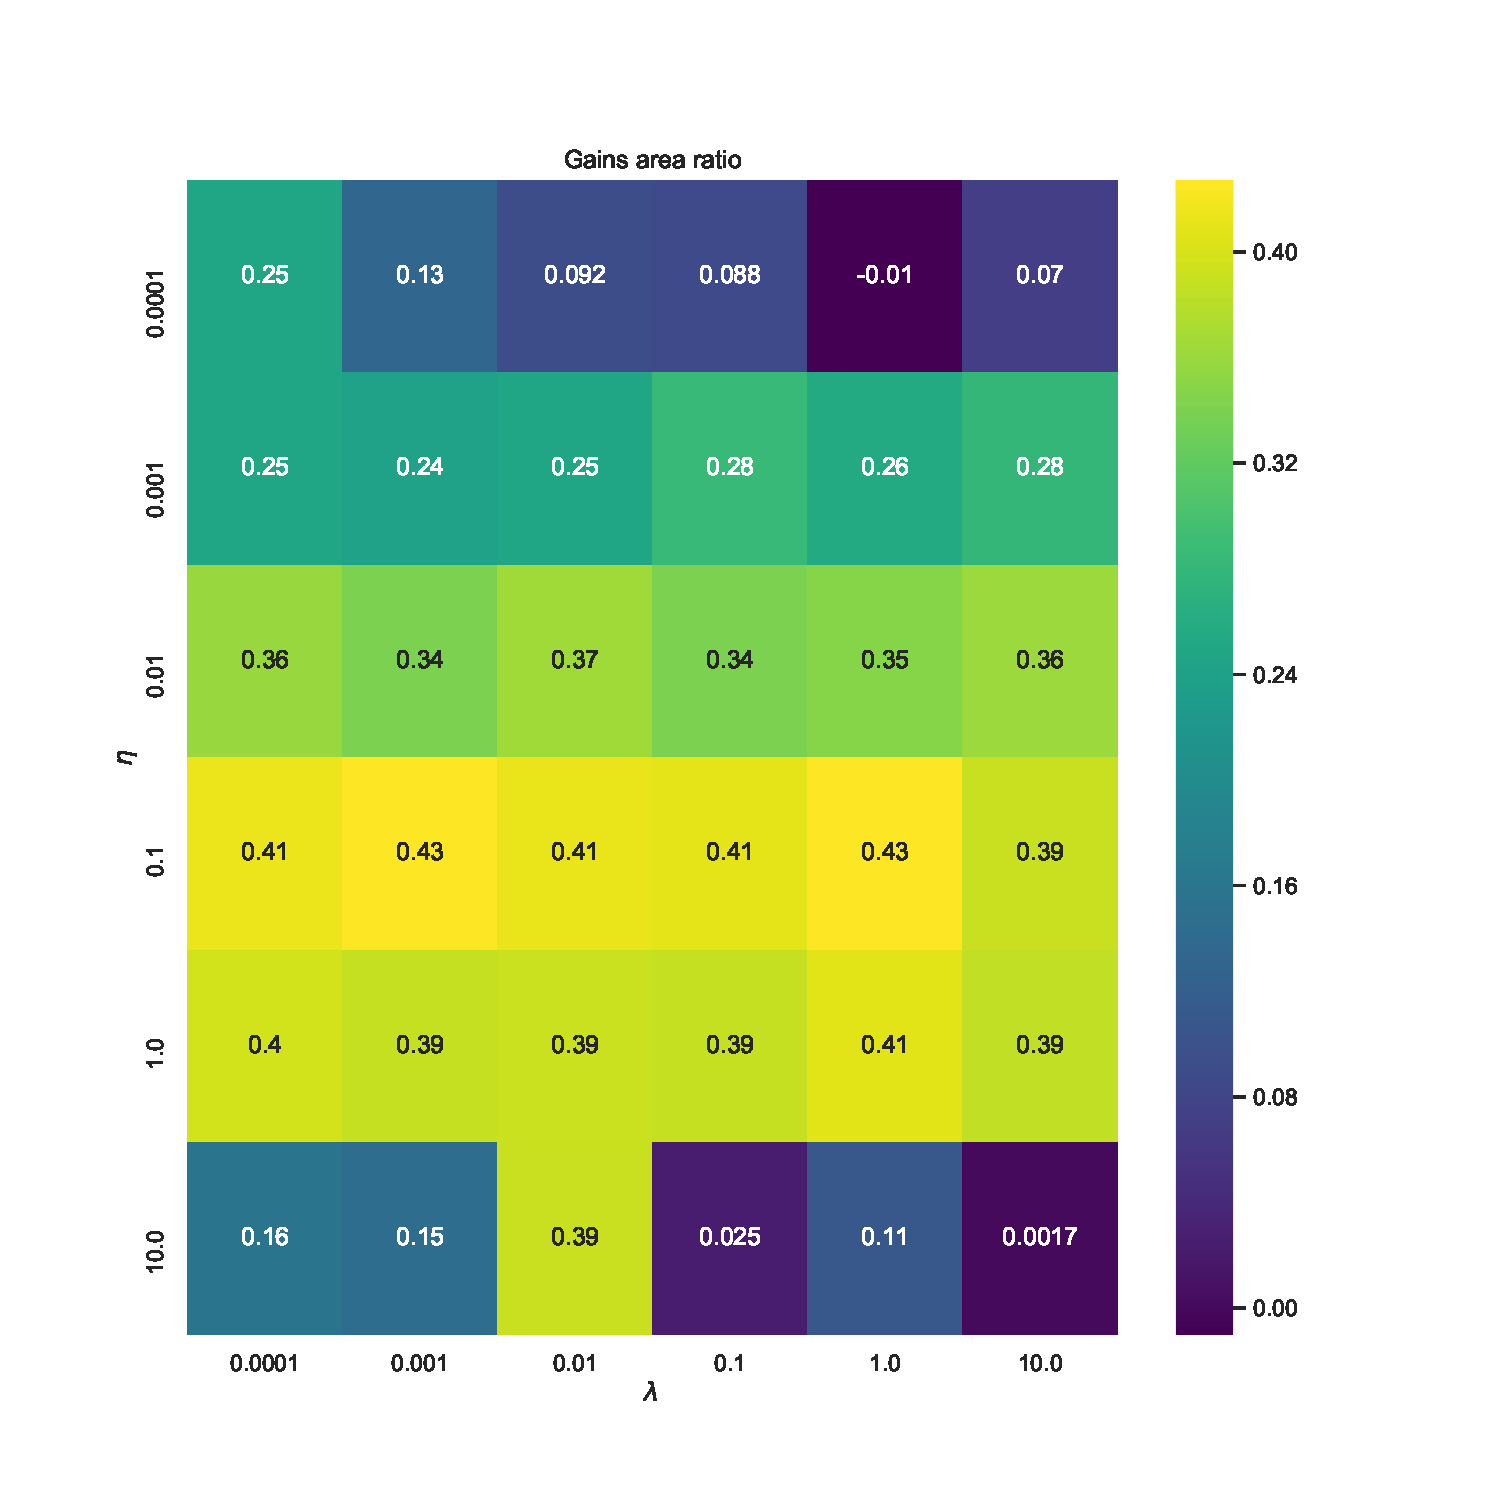
\includegraphics[scale=0.5]{../Results/CC_NN_gridsearch/gridsearch_NN_area.pdf} 
        \caption{Gridsearch showing area ratio score for a number of values of $\eta$ and $\lambda$, using $1000$ epochs over a batch size of $1000$. }
        \label{fig:NN1_grid_eta}   
\end{figure}  

\subsubsection{Neural network on Franke's Frunction}
\paragraph{Table \ref{table:mse_NN_p1}} shows a comparison of averaged MSE for the neural network and OLS on ($30 \times 30)$ Franke's function generated data sets with noise $\sim N(0,0.3)$. The table indicates that the neural network produces an MSE that is up to $26$ orders of magnitude larger than what the OLS from scikit-learn produces.


\begin{table}[h!]
\begin{center}
\begin{tabular}{lllll}
\hline
 Model & Validation & $\eta$  & $\lambda$  & MSE       \\
\hline
 Neural Network & Training (no split)   & $0.01$& $0.17$  & $2 \times 10^{-5}$ \\
 Neural Network & Test ($0.25$ of the data) & $0.31$& $0.01$  & $3 \times 10^{-5}$ \\
 OLS & Training (no split)   & - & -  & $6 \times 10^{-30}$\\
 OLS & Test ($0.25$ of the data)  & - & -  & $3 \times 10^{-31}$ \\
\hline
\end{tabular}
\end{center}
\caption{MSE after gridsearch for $\eta$ and $\lambda$ on ($30 \times 30)$ Franke's function generated data sets with noise $\sim N(0,0.3)$ for the neural network ($1000$ epochs, batch size $50$), compared with MSE for OLS using scikit-learn}
\label{table:mse_NN_p1}
\end{table}

\section{Discussion of results} \label{Section_Discussion_of_results}
\subsection{Implementation, testing, and evaluation}
The accuracy score of the logistic regression model on the raw credit card data (with one-hot encoding and outlier removal) is $0.78$, a deceivingly high score, considering that the area ratio score is $0.00$. This indicates that that the model is classifying all the test data as $0$ ($1$ being defaulting on payment) - which the confusion matrix  \hyperref[APP_1]{(see appendix 1)} confirms. The discrepancy in evaluation scores, and the gains chart (\ref{fig:logreg_no_pp}), shows that accuracy is not necessarily a meaningful measurement on model performance. Additionally, having performed no better than a random classifier suggest that additional pre-processing of data is necessary, which is not surprising considering that only $22\%$ of the entries after outlier removal have $y=1$, ie. the data set is considerably skewed. As indicated in table \ref{table:PP_scores}, scaling is by far the most important data pre-processing in the case of credit card data - which may be due to the wide range of predictor values - the highest un-scaled value is $1684258$, while the lowest are $0$. The best performance evaluated by area ratio ($0.46$) is obtained with outlier removal, one-hot, scaling, smote. Area ratio score of $0.46$ slightly outperforms similar analysis from \cite{YCCC} ($0.44$), which may be due to factors such as split ratio. Corresponding performance when using stochastic gradient decent and sci-kit were $0.44$ and $0.33$, respectively. 

\subsection{Neural network on credit card data}
The first grid search (figure \ref{fig:NN1_grid_epoch}) points to $500$ epochs over batches of size $500$, or $1000$ by $1000$ for $+eta=0.1$ and $\lambda=0.1$ (area ratio score = $0.42$), and shows a trend for intermediate batch sizes and epochs for (relatively) low values of the regularization ($\lambda$). The trend visible in  figure \ref{fig:NN1_grid_epoch_highl}, would suggest that a low number of epochs and large batch sizes (again, relatively speaking) produce the best results (area ratio score = $0.43$). This could indicate that higher values of $\lambda$ allow for a larger number of epochs, as the model does not over-fit as easily with severe regularization penalty, thus does not display a drop in area ratio score on test data. The two best epoch and batch size combinations in for low $\lambda$ would also suggest this. Figure \ref{fig:NN1_grid_eta} exemplifies however that the choice of $\lambda$ is not necessarily as directly linked to the number of epochs and batch size as the above discussion would suggest. The two parameter pairs of $\eta=0.1$ and $\lambda=0.001$, and $\eta=0.1$ and $\lambda=1.0$ with the highest area ratio score ($0.43$) for $1000$ epochs and batch size $1000$, may suggest that some values of epochs and batch size have several optimal combinations for learning rate and regularization - suggesting further that choosing suitable combinations of the four parameters is challenging at best, and may require more permutations than what this project shows. Additionally, comparison of the figures shows a discrepancy for $\eta=0.1,\lambda=1.0,epochs=1000,batche \textit{ }=1000$; figure \ref{fig:NN1_grid_epoch_highl} yields a score of $0.41$, while  figure \ref{fig:NN1_grid_eta} yields $0.43$ - which may indicate some error in implementation, or alternatively display the stochastic properties of SGD and/or the splitting and smote. The neural network appears to predict on par with logistic regression, albeit this may not be the case if more layers and implemented and/or better parameter adjustment is carried out. The paper by  I-Cheng Yeh and Che-Hui Lien \cite{YCCC} reports area ratio scores of $0.54$ for neural networks on the credit card data, which very strongly suggests that further improvement on the current implementation is achievable.

\subsection{Neural network on Franke's Frunction}
As table \ref{table:mse_NN_p1} clearly indicates; the neural network using one hidden layer does not perform nearly as well as OLS from scikit-learn, with MSE that up to $26$ orders of magnitude larger than what the OLS  on a ($30 \times 30)$ Franke's function generated data set with noise $\sim N(0,0.3)$, both using validation sets and not. This may either indicate an ineptitude for neural networks in general, although the (relatively) high MSE is assumed to not be representative of neural networks as a whole. A more likely option is either failure to find suitable parameters (epochs, batch size, $\eta$ and $\lambda$), one hidden layer being inadequate, or implementation error that was not triggered by initial testing, or a combination of these. As such, further testing is required in order to establish neural network aptitude for quantitative prediction. This project is unable to make any certain conclusions on the matter other than that the current implementation with one layer appears to favor OLS for predicting terrain.

\section{Conclusions} \label{Section_Conclusions}
This project concludes that accuracy is unsuited as a measurement of prediction quality in categorical modeling for skewed data sets, having calculated an accuracy score of $0.78$ for a model performing equivalent to a random classifier on the credit card data.

\bibliography{ref}
\bibliographystyle{plain}


\begin{appendices}
\section*{Appendix 1.} \label{APP_1}

\subsection*{Initial test on cancer data}
\paragraph{GD - Own model:}
Accuracy: 0.97 Area score: 0.99 
\begin{equation}
confusion=\begin{bmatrix}
tn=63 & fp=2 \\
fn=3  &tp= 120 \\
\end{bmatrix}
\end{equation}

\paragraph{SGD - Own model:}
Accuracy: 0.96 Area score: 0.99 
\begin{equation}
confusion=\begin{bmatrix}
tn=61 & fp=4 \\
fn=3  &tp= 120 \\
\end{bmatrix}
\end{equation}

\paragraph{Sklearn model:}
Accuracy: 0.97 Area score: 0.90 
\begin{equation}
confusion=\begin{bmatrix}
tn=61 & fp=4 \\
fn=2  &tp= 121 \\
\end{bmatrix}
\end{equation}


\subsection*{Credit card data, no pre-processing}
\begin{equation}
confusion=\begin{bmatrix}
tn=7591 & fp=0 \\
fn=2178  &tp= 0 \\
\end{bmatrix}
\end{equation}

\subsection*{Implementation test of NN}
See figre \ref{fig:NN_cost_initial}
\begin{figure}[!h]
        \centering 
         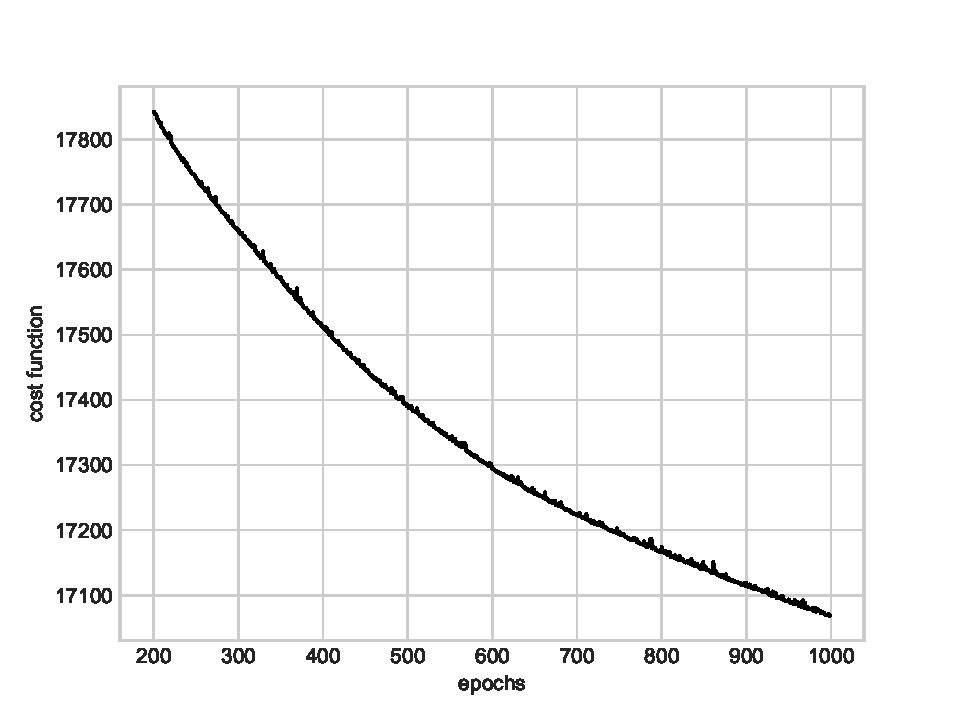
\includegraphics[scale=0.5]{../Results/CC_NN_initial/cost_NN.pdf} 
        \caption{Plot of cost function for NN for initial implementation test }
        \label{fig:NN_cost_initial}   
\end{figure}  

\subsection*{Iterations and batch size NN on credit card data}
\begin{table}[h!]
\begin{center}
\begin{tabular}{lll}
\hline
 Epochs  & Batch size & Area ratio score   \\
\hline
$2000$ & $1000$ &
$0.39$ \\
$1500$ & $2000$ &
$0.407$ \\
$1500$ & $500$ & 
$0.408$ \\
$1000$ & $1000$ &
$0.41$ \\
$600$ & $200$& 
$0.4$\\
\hline
\end{tabular}
\end{center}
\caption{Neural network on credit card data; area ratio score as functions of epochs and batch size using $\eta=0.1$ and $\lambda=0.0$}
\label{table:NN_epochs_batches}
\end{table}
\end{appendices}
\end{document}